Un organisme certificateur est missionné pour évaluer deux appareils de chauffage, l'un d'une marque A et l'autre d'une marque B.

\begin{center}
\textit{Les parties $1$ et $2$ sont indépendantes.}
\end{center}

\subsection*{Partie 1 : appareil de la marque A}

À l'aide d'une sonde, on a mesuré la température à l'intérieur du foyer d'un appareil de la marque $A$.

On a représenté, ci-dessous, la courbe de la température en degrés Celsius à l'intérieur du foyer en fonction du temps écoulé, exprimé en minutes, depuis l'allumage du foyer.

\begin{center}
	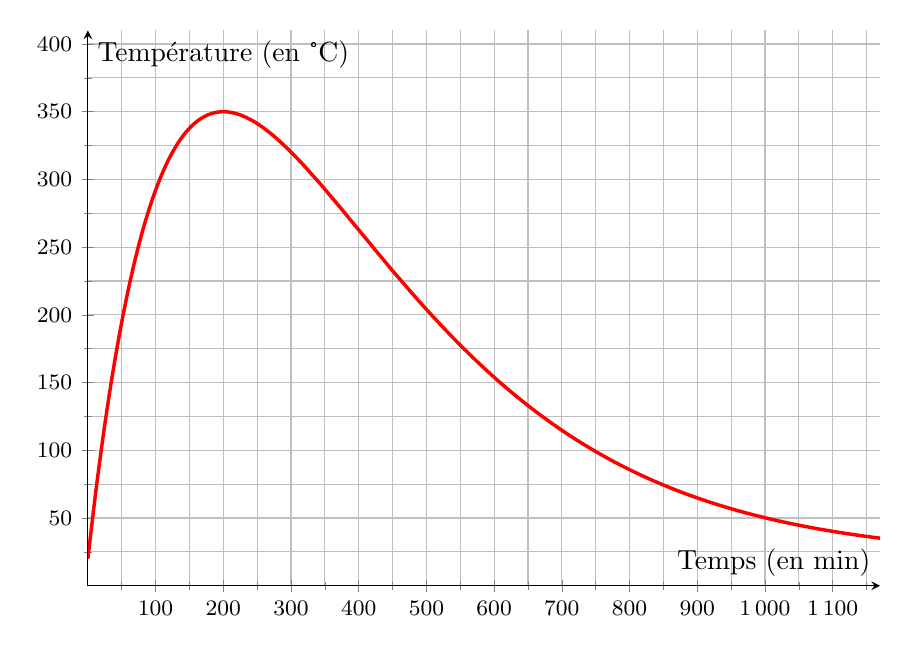
\begin{tikzpicture}
		\begin{axis}[/pgf/number format/.cd, use comma,/pgf/number format/set thousands separator={\,}, x={0.086mm}, y={0.172mm}, xmin=0, xmax=1170, ymin = 0, ymax=410, xtick distance=100, ytick distance =50,
			xlabel={Temps (en min)},ylabel={Température (en °C)},
			tick label style={font=\footnotesize}, minor tick num = 1, grid=both, axis lines =center]
			\addplot [line width=1.25pt,color=red,smooth,samples=100,domain= 0:1170 ]{20+330*x*exp(-0.005*x)/73.58};
			\node[below left] at (axis cs: 0,0) {{\footnotesize 0}};
		\end{axis}
	\end{tikzpicture}
\end{center}

Par lecture graphique :

\begin{enumerate}
	\item Donner le temps au bout duquel la température maximale est atteinte à l'intérieur du foyer.
	\item Donner une valeur approchée, en minutes, de la durée pendant laquelle la température à l'intérieur du foyer dépasse $300$~\ensuremath{^\circ} C.
	\item On note $f$ la fonction représentée sur le graphique.

	Estimer la valeur de \quad $\displaystyle\dfrac{1}{600} \int_{0}^{600} f(t) \d t$.\quad Interpréter le résultat.
\end{enumerate}

\subsection*{Partie 2 : étude d'une fonction}
Soit la fonction $g$ définie sur l'intervalle $[0~;~+ \infty[ $ par :

\[g(t) = 10 t \e^{-0,01 t} + 20.\]

\begin{enumerate}
	\item Déterminer la limite de $g$ en $+ \infty$.
	\item \begin{enumerate}
		\item Montrer que pour tout $t \in [0~;~+ \infty[,\quad g'(t)=(-0,1 t + 10) \e^{- 0,01 t}$.
		\item Étudier les variations de la fonction $g$ sur $[0~;~+ \infty[$ et construire son tableau de variations.
	\end{enumerate}
	\item Démontrer que l'équation $g(t) = 300$ admet exactement deux solutions distinctes sur [$0~;~+ \infty[$. En donner des valeurs approchées à l'unité.
	\item À l'aide d'une intégration par parties, calculer \quad $\displaystyle \int_{0}^{600} g(t) \:\text{d}t$.
\end{enumerate}

\subsection*{Partie 3 : évaluation}
Pour un appareil de la marque B, la température en degrés Celsius à l'intérieur du foyer $t$ minutes après l'allumage est modélisée sur $[0~;~600]$ par la fonction $g$.

L'organisme certificateur attribue une étoile par critère validé parmi les quatre suivants :

\begin{itemize}
\item Critère 1 : la température maximale est supérieure à $320~$\ensuremath{^\circ} C.
\item Critère 2 : la température maximale est atteinte en moins de 2 heures.
\item Critère 3 : la température moyenne durant les 10 premières heures après l'allumage dépasse $250$~\ensuremath{^\circ} C.
\item Critère 4 : la température à l'intérieur du foyer ne doit pas dépasser $300$~\ensuremath{^\circ} C pendant plus de 5 heures.
\end{itemize}

Chaque appareil obtient-il exactement trois étoiles ? Justifier votre réponse.
